\documentclass[handout, 10pt, aspectratio=43]{beamer}
%\documentclass[10pt, aspectratio=43]{beamer}
\usepackage[english]{babel}
\usepackage[backend=biber, style=numeric]{biblatex}
\bibliography{../report/ML-literature.bib}

\usepackage{amsthm}
\usepackage{animate}
\usepackage{mathtools}
\usepackage{physics}
\usepackage{calligra}
\usepackage{csquotes}
\usepackage{tensor}
\usepackage[thicklines]{cancel}
\usepackage{tcolorbox}
\usepackage{pstricks}
\usepackage{ulem}
%\usepackage[ngerman]{babel} % Language hyphenation and typographical rules
%\usepackage[backend=biber, style=numeric]{biblatex}

\setbeamersize{text margin left=0.5cm,text margin right=0.5cm}


\DeclareMathAlphabet{\mathcalligra}{T1}{calligra}{m}{n}
\DeclareFontShape{T1}{calligra}{m}{n}{<->s*[2.2]callig15}{}
\newcommand{\scriptr}{\mathcalligra{r}\,}
\newcommand{\boldscriptr}{\pmb{\mathcalligra{r}}\,}
\def\rc{\scriptr}
\def\brc{\boldscriptr}
\def\hrc{\hat\brc}
\newcommand{\ie}{\emph{i.e.}} %id est
\newcommand{\eg}{\emph{e.g.}} %exempli gratia
\newcommand{\rtd}[1]{\ensuremath{\left\lfloor #1 \right\rfloor}}
\newcommand{\dirac}[1]{\ensuremath{\delta \left( #1 \right)}}
\newcommand{\diract}[1]{\ensuremath{\delta^3 \left( #1 \right)}}
\newcommand{\e}{\ensuremath{\epsilon_0}}
\newcommand{\m}{\ensuremath{\mu_0}}
\newcommand{\V}{\ensuremath{\mathcal{V}}}
\newcommand{\prnt}[1]{\ensuremath{\left(#1\right)}} %parentheses
\newcommand{\colch}[1]{\ensuremath{\left[#1\right]}} %square brackets
\newcommand{\chave}[1]{\ensuremath{\left\{#1\right\}}}  %curly brackets

\useoutertheme{infolines}
\useinnertheme{rectangles}
\usefonttheme{professionalfonts}


%\definecolor{blue}{RGB}{0, 169, 224}
\definecolor{blue}{RGB}{0, 130, 224}
\definecolor{gray}{HTML}{ffffff}
\definecolor{yellow}{HTML}{f0be52}
\definecolor{lightblue}{RGB}{89, 199, 254}

\renewcommand{\CancelColor}{\color{blue}}

\makeatletter
\newcommand{\mybox}[1]{%
  \setbox0=\hbox{#1}%
  \setlength{\@tempdima}{\dimexpr\wd0+13pt}%
  \begin{tcolorbox}[colback=blue,colframe=blue,boxrule=0.5pt,arc=4pt,
      left=6pt,right=6pt,top=6pt,bottom=6pt,boxsep=0pt,width=\@tempdima]
    \textcolor{black}{#1}
  \end{tcolorbox}
}
\makeatother

\usecolortheme[named=blue]{structure}
\usecolortheme{sidebartab}
\usecolortheme{orchid}
\usecolortheme{whale}
\setbeamercolor{alerted text}{fg=yellow}
\setbeamercolor{block title alerted}{bg=alerted text.fg!90!black}
\setbeamercolor{block title example}{bg=lightblue!60!black}
\setbeamercolor{background canvas}{bg=gray}
\setbeamercolor{normal text}{bg=gray,fg=black}

\setbeamertemplate{footline}
        {
      \leavevmode%
      \hbox{%
      \begin{beamercolorbox}[wd=.333333\paperwidth,ht=2.25ex,dp=1ex,center]{author in head/foot}%
        \usebeamerfont{author in head/foot}\insertshortauthor~~(\insertshortinstitute)
      \end{beamercolorbox}%
      \begin{beamercolorbox}[wd=.333333\paperwidth,ht=2.25ex,dp=1ex,center]{title in head/foot}%
        \usebeamerfont{title in head/foot}\insertshorttitle
      \end{beamercolorbox}%
      \begin{beamercolorbox}[wd=.333333\paperwidth,ht=2.25ex,dp=1ex,center]{date in head/foot}%
        \usebeamerfont{date in head/foot}\insertshortdate{}%\hspace*{2em}

    %#turning the next line into a comment, erases the frame numbers
        %\insertframenumber{} / \inserttotalframenumber\hspace*{2ex} 

      \end{beamercolorbox}}%
      \vskip0pt%
    }


\setbeamertemplate{blocks}[rectangle]
\setbeamercovered{dynamic}

\setbeamertemplate{section page}
{
	\begin{centering}
		\begin{beamercolorbox}[sep=27pt,center]{part title}
			\usebeamerfont{section title}\insertsection\par
			\usebeamerfont{subsection title}\insertsubsection\par
		\end{beamercolorbox}
	\end{centering}
}

%\setbeamertemplate{subsection page}
%{
%	\begin{centering}
%		\begin{beamercolorbox}[sep=12pt,center]{part title}
%			\usebeamerfont{subsection title}\insertsubsection\par
%		\end{beamercolorbox}
%	\end{centering}
%}

\newcommand{\hlight}[1]{\colorbox{violet!50}{#1}}
\newcommand{\hlighta}[1]{\colorbox{red!50}{#1}}

\settowidth{\leftmargini}{\usebeamertemplate{itemize item}}
\addtolength{\leftmargini}{\labelsep}

\usepackage{ragged2e}
\usepackage{cases}

\mathcode`\*="8000
{\catcode`\*\active\gdef*{\cdot}}

\usepackage[]{siunitx}

\sisetup{per-mode=fraction, locale = US, expproduct = cdot }
\sisetup{locale = UK}							%	Automatische Einstellung der Ausgabe für bestimmte Regionen (UK, US, DE, FR, ZA)
\sisetup{
	per-mode=fraction,
	fraction-function=\tfrac
}
\DeclareSIUnit\Hy{H}
\DeclareSIUnit\hPa{hPa}
\DeclareSIUnit\Torr{Torr}
\DeclareSIUnit\T{T}
% FLORIAN
\usepackage{graphics}
\def\R{{\mathbb{R}}}
\def\N{{\mathbb{N}}}
\def\C{{\mathbb{C}}}
\def\K{{\mathbb{K}}}
\def\Q{{\mathbb{Q}}}
\def\Z{{\mathbb{Z}}}
\def\O{{\mathcal{O}}}
\def\Pot{{\mathcal{P}}}
\def\P{{\mathbb{P}}}
\def\D{{\mathcal{D}}}
\def\B{{\mathcal{B}}}
\def\U{{\mathcal{U}}}
\def\F{{\mathcal{F}}}
\def\M{{\mathcal{M}}}
\def\E{{\mathbb{E}}}
\def\EEE{{\mathcal{E}}}
\def\Cov{{\mathbb{C}\mathrm{ov}}}
\def\Var{{\mathbb{V}\mathrm{ar}}}
\def\V{{\mathbb{V}}}
\def\ND{{\mathcal{N}}}
\def\essup{{\mathrm{ess \;sup}}}

\usepackage{multirow}
\usepackage{booktabs}
\usepackage{subfigure}

\title{Predicting a vehicles velocity using dashcam footage} %->->->->-> Check hyperref title <-<-<-<-<-
\subtitle{A deep learning approach}
\author[Florian Wolf, Franz Herbst]{Florian Wolf, Department of Mathematics and Statistics\\Franz Herbst, Department of Physics}
\institute[Universität Konstanz]{
    Machine Learning using \sout{Matlab} Python \\
    Universität Konstanz
} %You can change the Institution if you are from somewhere else
\date{\today}
%\logo{\includegraphics[width= 0.2\textwidth]{images/a-logo.png}}

\begin{document}
    \RaggedRight
    \frame{\titlepage}
    
    \begin{frame}{Table of content}
        \tableofcontents
    \end{frame}
    
    \section{Motivation and initial Dataset}


\begin{frame}{The \enquote{comma ai speed challenge}\footnote{https://github.com/commaai/speedchallenge}}
	\textbf{Motivation}
	\begin{itemize}
		\item autonomous driving is currently one of the most prominent problems in machine learning
		\item but quite hard to set up on a desktop pc
		\item predicting a vehicles velocity from video footage is a related but also much more simplified task
	\end{itemize}
	\pause
	\textbf{Initial Dataset:}
	\begin{itemize}
		\item training video with 20400 frames (20 fps)
		\item data file with velocity of the car at each frame
		\item test video with 10798 frames (20 fps)
	\end{itemize}
	\pause
	\textbf{Evaluation:}
	\begin{itemize}
		\item the mean squared error (MSE) is used to measure performance
		\begin{align*}
			\mathcal{L} = \sum_i (p(x_i) - y_i)^2
		\end{align*}
	\end{itemize}
\end{frame}

\begin{comment}

\begin{frame}{The \enquote{comma ai speed challenge}\footnote{https://github.com/commaai/speedchallenge}}
\textbf{Motivation}
\begin{itemize}
\item HERE ARE SOME MOTIVATIONAL WORDS NEEDED
\end{itemize}
\textbf{Data collection:}
\begin{itemize}
\item \enquote{comma ai speed challenge} provides two videos:
\setbeamertemplate{itemize items}[circle]
\begin{itemize}
\item Train video: 24000 frames, shoot at 20 frames per second, including ground truths
\item Test video: 10798 frames, shoot at 20 frames per second, no ground truths, used to applications
\end{itemize}
\item Split train video after 80$\%$ with hard cut off (ability the generalize), to get train and test datasets
\end{itemize}
\textbf{Initial assumptions}
\begin{itemize}
\item<+-> Use mean squared error (MSE) as a performance measure
\item<+-> How to evaluate a prediction? Assumptions:
\setbeamertemplate{itemize items}[circle]
\begin{itemize}
\item MSE $\leq 10$: good
\item MSE $\leq 5$: better
\item MSE $\leq 3$: correct
\end{itemize}
\end{itemize}
\end{frame}

\end{comment}
    \section{Analysis of the dataset}

\begin{frame}{Analysis of the dataset}
	\textbf{Video data:}
	\begin{itemize}
		\item<+-> frame size of $(640,480,3)$ pixels
		\item<+-> cut off last 60 pixels, to remove black frame inside the car
		\item<+-> sample down the frame to half its size, to reduce computation time
	\end{itemize}
	
	\begin{columns}[t]
		\begin{column}{.45\textwidth}
			\begin{center}
				\only<1->{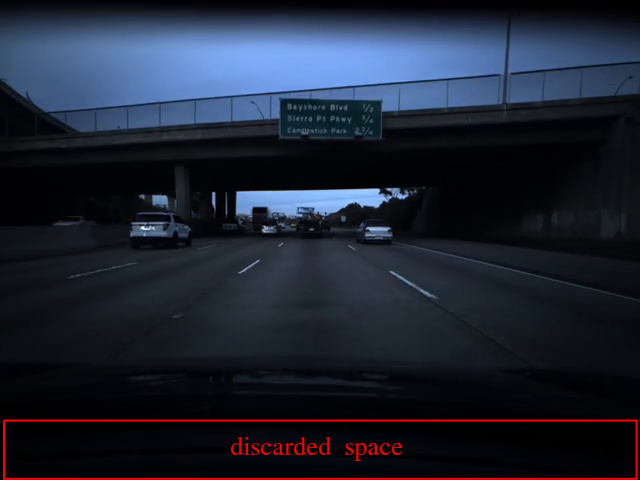
\includegraphics[width=\linewidth]{./imgs/frame2_evaluated.png}}
				\small{Original frame}
			\end{center}
		\end{column}
		\begin{column}{.45\textwidth}
			\begin{center}
				\only<3->{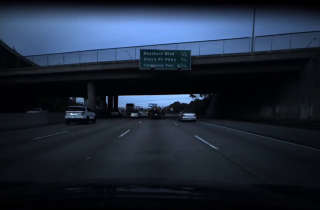
\includegraphics[width=\linewidth]{./imgs/frame2_cut_sampled.png}}
				\small{Cut off the last 60 pixels, downsampled}
			\end{center}
		\end{column}
	\end{columns}
\end{frame}

\begin{frame}{Analysis of the dataset}
	\begin{columns}[c]
		\begin{column}{.55\textwidth}
			\textbf{Splitting of the dataset}
			\begin{itemize}
				\item<+-> Initial splitting: hard cut off after $80\%$ of the frames
				\item<+-> Situational splitting: divide dataset into blocks of different driving scenarios,
				splitting with $80\%$ test and $20\%$ validation data on each
%				\setbeamertemplate{itemize items}[circle]
%				\begin{itemize}
%					\item divide dataset into blocks of different categories
%					\item splitting with $80\%$ test and $20\%$ validation data on each
%				\end{itemize}
			\end{itemize}
			\pause
			\textbf{Evaluation:}
			\begin{itemize}
				\item<+-> variance $\sqrt{\mathcal{L}} \gtrsim 16$: no fitting
				\item<+-> $10 \lesssim \sqrt{\mathcal{L}} \lesssim 16$: average velocity fitted
				\item<+-> $5 \lesssim \sqrt{\mathcal{L}} \lesssim 10$: qualitative detection
				\item<+-> $1 \lesssim \sqrt{\mathcal{L}} \lesssim 5$: quantitative detection
				\item<+-> $\sqrt{\mathcal{L}} \lesssim 1$: perfect detection
			\end{itemize}
		\end{column}
		\begin{column}{.45\textwidth}
			\begin{center}
				\only<1->{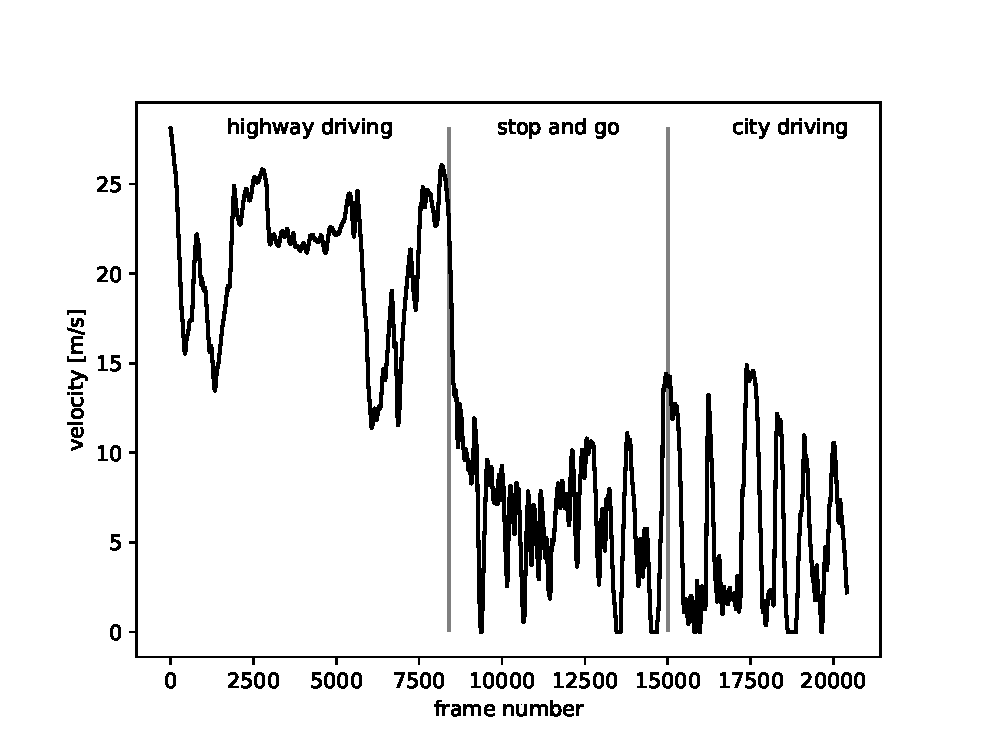
\includegraphics[width=0.85\textwidth, height=0.34\textheight]{./imgs/plot_speed_time_new_splitting.eps}
				{\footnotesize driving situations in v-t-plot}}
				\only<5->{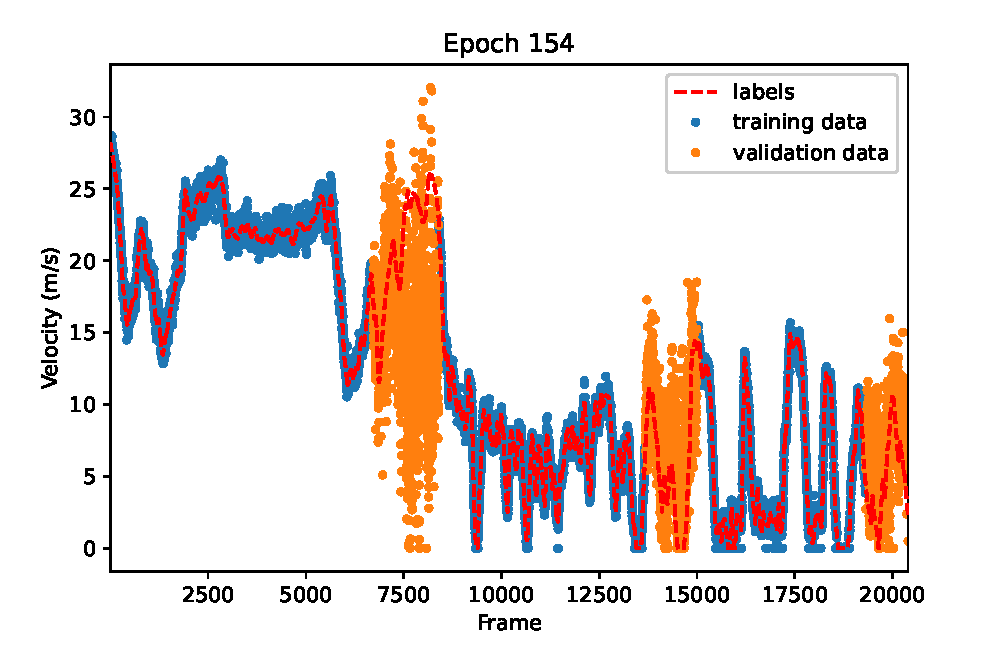
\includegraphics[width=0.85\textwidth]{./imgs/example_performance.eps}
				{\footnotesize example performance on training set \\ training: $\sqrt{\mathcal{L}}=0.4$, test: $\sqrt{\mathcal{L}}=6.3$}}
			\end{center}
		\end{column}
	\end{columns}
\end{frame}
    \section{Preprocessing using optical flow}

\begin{comment}
\begin{frame}{Preprocessing}
    \begin{itemize}
    \item Frame size of $(640,480,3)$ pixels
    \item Cut off last 60 pixels, to remove black frame inside the car
    \item Sample down the frame to half its size, due to computational limitations
    \end{itemize}

\begin{columns}[t]
\begin{column}{.45\textwidth}
\begin{center}
\only<1->{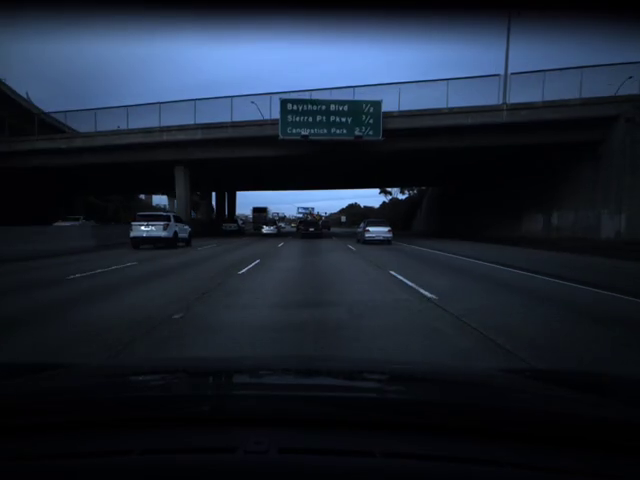
\includegraphics[width=\linewidth]{./imgs/frame2_original.png}}
\small{Original frame}
\end{center}
\end{column}
\begin{column}{.45\textwidth}
\begin{center}
\only<1->{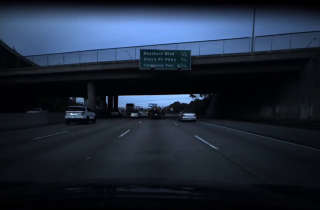
\includegraphics[width=\linewidth]{./imgs/frame2_cut_sampled.png}}
\small{Cut off the last 60 pixels, downsampled}
\end{center}
\end{column}
\end{columns}
\end{frame}
\end{comment}

\begin{frame}{Optical flow using \enquote{Farneback pyramid method}\cite{Farneback2003}}

\begin{itemize}
\item Global method to solve the optical flow equation
\begin{align*}
\partial_x f \cdot V_x + \partial_y f \cdot  V_y + \partial_t f  = 0
\end{align*}
for an image sequence $(f_t)_t$ with $f_t : \Omega \to \R^3$, for all $t$, and the (dense) flow field $V : \Omega \to \R^2, \omega \mapsto (V_x(\omega), V_y(\omega))$.
\item Uses a downsampling pyramid, to solve the equation for different resolutions of the image
\item Parameters for the Farneback method
\begin{align*}
\text{pyramid levels} &:= 3\\
\text{pyramid scaling} &:= 0.5\\
\text{window size} &:= 6\\
\text{SD of the gaussian filter} &:= 1.1
\end{align*}
\item Result: \textbf{Flow field with $(160,105,3)$ pixels}
\end{itemize}
\end{frame}

\begin{frame}{Visualization of the flow field}
\begin{itemize}
\item Flow field is a two-dimensional vector field
\item RGB representation via
\setbeamertemplate{itemize items}[circle]
\begin{itemize}
\item Transform flow field into polar coordinates $(V_x,V_y) \overset{\simeq}{\mapsto} (r, \varphi)$
\item Normalize magnitudes $r$ for the third channel
\item Values of the second channel are all set to 255
\item Multiply angle $\varphi$ by factor $\frac{180}{2\pi}$ for the first channel
\end{itemize}
\item Sample down the resolution again to speed up the training
\end{itemize}

\begin{columns}[t]
\begin{column}{.45\textwidth}
\begin{center}
\only<1->{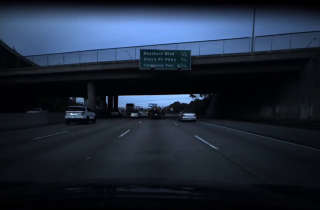
\includegraphics[width=0.85\linewidth]{./imgs/frame2_cut_sampled.png}}
\small{\\Input frame}
\end{center}
\end{column}
\begin{column}{.45\textwidth}
\begin{center}
\only<1->{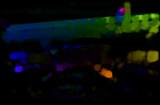
\includegraphics[width=0.85\linewidth]{./imgs/frame2_flow_field.png}}
\small{\\Corresponding flow field}
\end{center}
\end{column}
\end{columns}

\end{frame}


    \section{Method selection and architecture}

\begin{frame}{Convolutional neural network and initial architecture}
	\begin{columns}[c]
		\begin{column}{0.55\textwidth}
			\textbf{Method selection}
			\begin{itemize}
				\item<+-> speed prediction is a non-linear regression task $\Rightarrow$ neural network
				\item<+-> task involves feature extraction $\Rightarrow$ convolutional neural network (CNN)
			\end{itemize}
			\textbf{Initial architecture}
			\begin{itemize}
				\item<+-> using paper of \textit{NVIDIA} work group \cite{NVIDIA2016} of a CNN for self-driving cars adapted on our initial data
				\item<+-> enough complexity and layers to handle the task and lots of possibilities to fine-tune it
				\item<+-> Initial results with the raw model: $\mathcal{L} < 3$ on the training set and about $\mathcal{L} = 18-20$ on the test set\\
				$\Rightarrow$ Improvements needed
			\end{itemize}
		\end{column}
		\begin{column}{0.4\textwidth}
			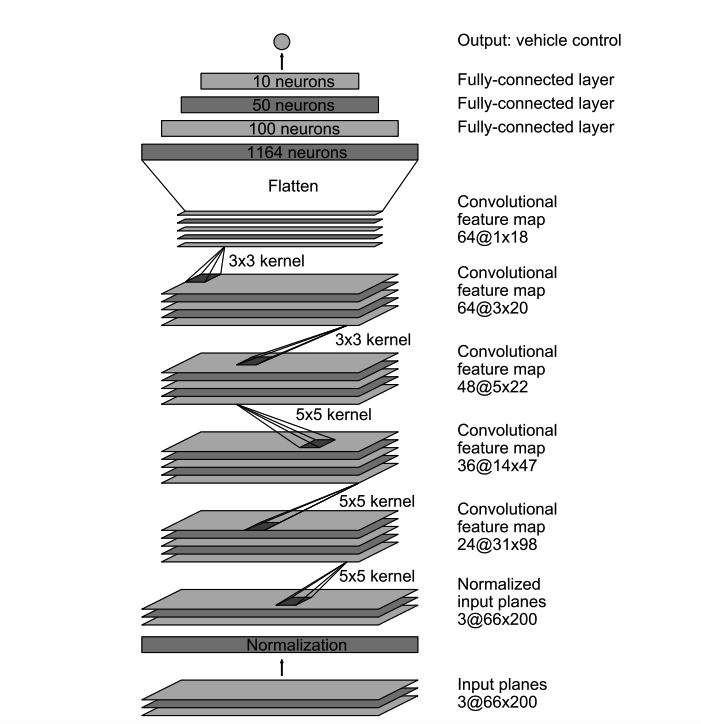
\includegraphics[width=\textwidth]{./imgs/NetworkOriginal.png}
			{\footnotesize Original architecture of the \textit{NVIDIA} paper \cite{NVIDIA2016}}
		\end{column}
	\end{columns}
\end{frame}

\begin{comment}
\begin{frame}[plain]
\begin{figure}
\centering
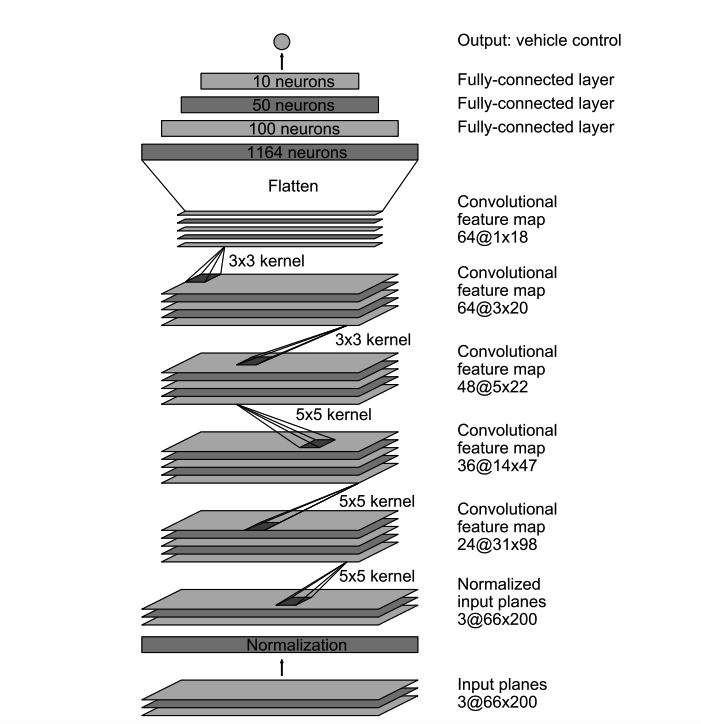
\includegraphics[scale=0.3]{./imgs/NetworkOriginal.png}
\caption{Original architecture of the NVIDIA paper \cite{NVIDIA2016}.}
\end{figure}
\end{frame}
\end{comment}
    \section{Fine-tuning of the model}
\subsection{Initial tuning}

\begin{frame}{Batch Normalization, Dropout layers, activation function and pooling}
\begin{itemize}
\item Batch normalization to speed up the training \cite{BatchNorm2015}
\item Initial activation function: $\mathrm{ReLu}: \mathbb{R} \to \mathbb{R}_0^+, x \mapsto \max\{0,x\}$, still MSE of over 15 on the testing 
set, less then 2 on the training set\\
$\Rightarrow$ Overfitting problems
\item Found paper about dropout layers \cite{Dropout2014} to reduce overfit
%build in one with dropout probability $p=0.5$
\item Solve problems of dead neurons using
\begin{align*}
\mathrm{leakyReLU} : \mathbb{R} \to \mathbb{R}, x \mapsto \begin{cases}
x, x \geq 0\\
c \cdot x, x <0
\end{cases}
\end{align*}
with $c = 0.01$, MSE of around 11 on the testing set and less than 3 on the training set
\end{itemize}
\end{frame}
\subsection{Problems and possible solutions}
\begin{frame}{Problems}
We identified three possible problems for our poor results
\begin{enumerate}
\item Too complex model, as initially used for autonomous driving or insufficient amount of information put into the model
\item Brightnesses/illumination changes in the frames, therefore unstable calculations of the optical flow
\item Too ambiguous splitting, as the training and testing datasets represent totally different road traffic scenarios
\end{enumerate}
IMAGE OF THE SPEED DISTRIBUTION
\end{frame}


\begin{frame}{Possible solutions}
\begin{enumerate}
\item \textbf{Simplify model}: pooling layers (maximum and average pooling) to get more compression\\
\textbf{Siamese approach}: put flow field and raw frame into the model or put two consecutive frames into the model
\item \textbf{Add additional noise}: add noise before computing the optical flow filed, to get more invariance regarding illumination changes
\item \textbf{Different splitting}: get better ratio between different scenarios, by using different data splittings:
finer one and a more specific one based on the different road traffic situations in the video
\end{enumerate}
\end{frame}
\subsection{Simplified model}
\begin{frame}{Pooling layers (initial splitting)}
\begin{table}[!t]
\normalsize
\centering
\begin{tabular}{lcccc}
\toprule
\multirow{2}{*}{Initial splitting, 8 epochs}  & \multicolumn{2}{c}{$\mathrm{ReLU}$} & \multicolumn{2}{c}{$\mathrm{leakyReLU}$} \\
 & Train & Test & Train & Test\\
\midrule
No pooling & 2.85 & 12.08 & 2.45 & 10.75 \\
Max pooling & 5.62 & 11.82 & 5.52 & 10.29 \\
Max pooling (15 epochs) & - & - & \textbf{3.22} & \textbf{9.63} \\
Average pooling & 7.70 & 11.40 & 6.08 & 13.09\\
\bottomrule
\end{tabular}
\caption{MSE results of the network using different pooling strategies, one dropout layers, two different activation functions and 
the initial splitting. We trained each of the models for eight epochs.}
\end{table}
\end{frame}
\subsection{Siamese approach: flow field and frame (new splitting)}
\begin{frame}{Siamese approach (new splitting)}
RESULTS ARE NEEDED :)
\end{frame}

	\section{Current and further work}
\subsection{Additional noise}
\begin{frame}{Contrast and brightness augmentation}
\begin{itemize}
\item Additional noise to frames \textbf{before} calculating the flow field.
\item Change the brightness and contrast of an image via
\begin{align*}
\text{frame}_{\mathrm{augmented}}(i,j) = \alpha(i,j) \cdot \text{frame}(i,j) + \beta(i,j)
\end{align*}
with functions $\alpha$ (contrast: $>1$ increase, $<1$ decrease) and $\beta$ (brightness).\\
To get some noise into the frames, we used
\begin{align*}
\alpha &\sim \mathcal{U}(0,1)+0.35\\
\beta &\sim \mathcal{U}(-5,35),
\end{align*}
where $\mathcal{U}(a,b)$ is the uniform distribution in an interval $[a,b]$ for $a < b$.
\end{itemize}
\end{frame}

\begin{frame}{Acquire more Data}
\begin{itemize}
	\item use mobile to create a video and track the velocity via GPS
	\item test run already worked
	\item data does not compare to the rest due to completely different brightness and angle
	\item but it would allow to create a greater data set with more training and labeld test data
\end{itemize}´
\end{frame}

\begin{frame}{Usage in real application}
	\begin{itemize}
		\item if we have good model we have written method that reads video and predicts velocity
		\item we reach 30 fps which is faster than the 20 fps of the video so life prediction would be possible
	\end{itemize}
\end{frame}

\begin{frame}{Evaluation with the test video}
	\begin{itemize}
		\item rough check how model performs on unseen video with the same parameters
		\item no labels available so we can only compare key situations (stops, highway, ...)
		\item some models achieve at least a qualitative accordance with the video (hier noch ein Bild)
		\item best networks: altered original network and 
	\end{itemize}
\end{frame}
	\section{Summary and application ideas}

\begin{frame}{Usability in real world application}
	\begin{itemize}
		\item using a similar setup as for acquiring the test data it would be possible to achieve a live prediction
		\item to test our predictions we wrote a method reading a video and predicting the speed
		\item even with calculating the optical flow we reach speed of 30 fps $\Rightarrow$ life prediction would be possible
		\item at the moment there is no completely convincing model
		\item a lot of programming would be involved
	\end{itemize}
\end{frame}
    \begin{frame}{References} %default [allowframebreaks]
    	\nocite{*}
        \printbibliography
     \end{frame}
\end{document}

